\documentclass[10pt]{article}
\usepackage[a4paper,margin=0.9cm,top=0.7cm,bottom=0.7cm,columnsep=0.45cm]{geometry}
\usepackage[utf8]{inputenc}
\usepackage[T1]{fontenc}
\usepackage{lmodern}
\usepackage{microtype}
\usepackage{multicol}
\usepackage{booktabs}
\usepackage{xcolor}
\usepackage{hyperref}
\usepackage{tikz}
\usepackage{pgfplots}
\pgfplotsset{compat=1.17}
\usetikzlibrary{positioning,arrows.meta,calc}

\definecolor{ucblue}{RGB}{0,51,102}
\definecolor{ftorange}{RGB}{204,85,0}
\definecolor{toolgray}{RGB}{110,110,110}
\hypersetup{colorlinks=true,urlcolor=ucblue,linkcolor=ucblue}
\setlength{\parindent}{0pt}
\setlength{\parskip}{1.5pt}
\pagestyle{empty}
\newcommand{\head}[1]{\textbf{\color{ucblue}#1}\hspace{0.4em}}
\newcommand{\pendiente}[1]{\textcolor{red}{[PENDIENTE: #1]}}
\newcommand{\VideoURL}{\href{https://youtu.be/zXe4w0KGbcs}{youtu.be/zXe4w0KGbcs}}
\newcommand{\HFURL}{\href{https://huggingface.co/vicentesonez/sql4business-planificador-qlora}{huggingface.co/vicentesonez/sql4business-planificador-qlora}}
\newcommand{\LOSSCSV}{../results/deliverable4/adapter/loss.csv}

\begin{document}

\begin{center}
{\Large\bfseries\color{ucblue} SQL4Business: Deliverable 4 --- fine-tuning del Planificador}\\[1pt]
{\small Generative Artificial Intelligence (580694), Universidad de Concepci\'on}\\[1pt]
{\small Aredhel Jim\'enez, Bryan Riquelme, Guido Salazar, Vicente So\~nez}\\[1pt]
{\small C\'odigo: \href{https://github.com/aredhel-jmze/Asistente-SQL-4-Business}{github.com/aredhel-jmze/Asistente-SQL-4-Business}
\quad$\vert$\quad Adaptador: \HFURL \quad$\vert$\quad Video: \VideoURL}
\end{center}

\vspace{-6pt}
\begin{center}
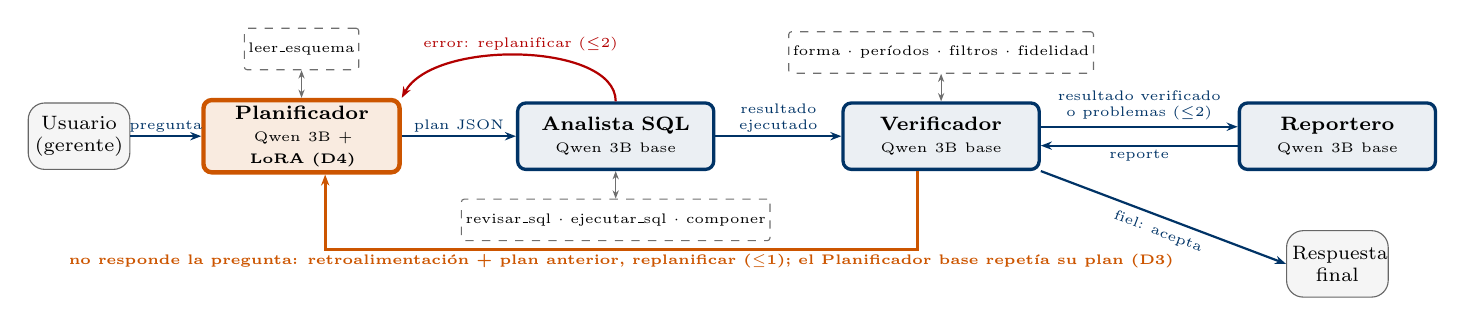
\begin{tikzpicture}[
  font=\scriptsize,
  agent/.style={draw=ucblue, fill=ucblue!8, very thick, rounded corners=3pt, align=center, minimum height=2.4em, text width=2.35cm, inner sep=2pt},
  ft/.style={agent, draw=ftorange, fill=ftorange!12, line width=1.6pt},
  tool/.style={draw=toolgray, dashed, rounded corners=1pt, align=center, font=\tiny, inner sep=1.5pt, minimum height=1.5em},
  ext/.style={draw=black!60, fill=black!4, rounded corners=6pt, align=center, minimum height=2.4em, text width=1.15cm, inner sep=2pt},
  flow/.style={-{Stealth[length=4pt]}, thick, ucblue},
  back/.style={-{Stealth[length=4pt]}, thick, red!70!black},
  use/.style={{Stealth[length=3pt]}-{Stealth[length=3pt]}, toolgray},
  lab/.style={font=\tiny, inner sep=1pt, align=center}]
  \node[ext] (u) {Usuario\\(gerente)};
  \node[ft, right=0.9cm of u] (p) {\textbf{Planificador}\\{\tiny Qwen 3B + \textbf{LoRA (D4)}}};
  \node[agent, right=1.45cm of p] (a) {\textbf{Analista SQL}\\{\tiny Qwen 3B base}};
  \node[agent, right=1.6cm of a] (v) {\textbf{Verificador}\\{\tiny Qwen 3B base}};
  \node[agent, right=2.5cm of v] (r) {\textbf{Reportero}\\{\tiny Qwen 3B base}};
  \node[ext, below=0.75cm of r] (o) {Respuesta\\final};
  \node[tool, above=0.35cm of p] (t1) {leer\_esquema};
  \node[tool, below=0.35cm of a] (t3) {revisar\_sql $\cdot$ ejecutar\_sql $\cdot$ componer};
  \node[tool, above=0.35cm of v] (t5) {forma $\cdot$ períodos $\cdot$ filtros $\cdot$ fidelidad};
  \draw[flow] (u) -- node[lab, above] {pregunta} (p);
  \draw[flow] (p) -- node[lab, above] {plan JSON} (a);
  \draw[flow] (a) -- node[lab, above] {resultado\\ejecutado} (v);
  \draw[flow] ($(v.east)+(0,0.12)$) -- node[lab, above=1pt] {resultado verificado\\o problemas ($\leq$2)} ($(r.west)+(0,0.12)$);
  \draw[flow] ($(r.west)+(0,-0.12)$) -- node[lab, below] {reporte} ($(v.east)+(0,-0.12)$);
  \draw[flow] (v.south east) -- node[lab, below=2pt, sloped] {fiel: acepta} (o.west);
  \draw[use] (t1) -- (p); \draw[use] (t3) -- (a); \draw[use] (t5) -- (v);
  \draw[back] (a.north) .. controls +(0,0.75) and +(0.4,0.75) .. node[lab, above] {error: replanificar ($\leq$2)} (p.north east);
  \draw[back, ftorange, line width=1.2pt] ($(v.south)+(-0.3,0)$) -- ++(0,-1.0) -| node[lab, pos=0.25, below, text=ftorange] {\textbf{no responde la pregunta: retroalimentación + plan anterior, replanificar ($\leq$1); el Planificador base repetía su plan (D3)}} ($(p.south)+(0.3,0)$);
\end{tikzpicture}
\end{center}
\vspace{-9pt}
{\tiny Naranja: el agente ajustado (LoRA sobre el mismo modelo base; los otros tres usan los pesos base) y el ciclo que debía corregir. Por el comentario al D3, el Verificador revisa el resultado antes del Reportero y después la fidelidad del reporte. Prompts en \texttt{prompts/}.}

\vspace{-2pt}
\begin{multicols}{2}
\small

\head{Tarea, falla y continuidad.} La misma tarea (pregunta de negocio $\rightarrow$ consultas SQL
necesarias y reporte fiel), la misma falla diagnosticada en el D1 (planificar preguntas combinadas:
0/5 con prompting directo) y el mismo sistema de cuatro agentes del D3, con el Verificador antes del
Reportero (las 27 trazas del D3 dan los mismos planes y resultados con este orden), con el mismo modelo
(\texttt{Qwen2.5-Coder-3B-Instruct}, rev.\ \texttt{488639f}, NF4, greedy) y el mismo criterio de
evaluación (\textit{sql}, \textit{answer}, \textit{e2e}).

\head{Elección del agente: el Planificador.} En la corrida final del D3, las 4 preguntas que el
sistema falla (q04, q10, q12, q11-p) nacen en un plan del Planificador; el Analista, el Reportero y
el Verificador no originan ningún error. Además, en 4 de las 6 veces que el Verificador o el Analista
le devolvieron el plan con el motivo exacto (``growth\_pct needs the earlier period first'', ``the
question names `Alimentos'\,''), el Planificador devolvió \emph{el mismo SQL}. El D3 ya agotó el prompting
(few-shot, descomposición, controles del Verificador): detectar funciona, corregir no, porque con
greedy el sesgo por el orden en que la pregunta nombra los meses domina la retroalimentación. Por eso
se cambian los pesos: enseñar con ejemplos (a)~a ordenar los períodos por tiempo y no por mención, y (b)~a
\emph{usar} la retroalimentación del Verificador. El control mide si los mismos datos, dados como
prompt, bastan.

\head{Datos.} 1.282 pares (entrada, salida) para el rol del Planificador
(\texttt{data/finetune/}, regenerables con \texttt{scripts/build\_planner\_data.py}, semilla 4).
\textit{Entrada}: el prompt exacto que lee el Planificador en ejecución (esquema enriquecido,
técnicas del D3, pregunta). \textit{Salida}: el plan JSON correcto. \textit{Fuente}: plantillas de
preguntas (86\,\% español, 14\,\% inglés) sobre \texttt{business.db}, en 8 familias de operación.
\textit{Etiquetado}: ningún modelo escribe salidas; cada plan lo construye el código a partir de los
parámetros de la tarea, se ejecuta con las herramientas del Analista y se compara con un valor de
referencia calculado en Python sobre las tablas (0 discrepancias; se descartan empates).
883 ejemplos de \emph{plan} (51\,\% de los de crecimiento nombran primero el período posterior, como
q12) y 399 de \emph{reparación}: plan equivocado (7 tipos: orden invertido, filtro omitido, etc.)
+ la retroalimentación que produce la propia función del Verificador $\rightarrow$ plan correcto. \textit{Revisión}: además de verificar por
ejecución los 1.282 pares, se revisó a mano una muestra al azar de 60 (\texttt{revision\_manual.csv}):
60/60 correctos; 6 leen ``ventas'' como conteo (ver el caso de falla).
\textit{Separación}: de 4.737 tareas se eliminaron las 450 con la misma operación y resultado, un paso
numérico igual o similitud de 5-gramas $\geq 0{,}5$ con una pregunta de evaluación (máxima restante:
0,19). Train/dev (1.155/127) se separan por cálculo; un test lo comprueba.

\head{Entrenamiento.} QLoRA (\texttt{scripts/train\_planner.py}, bucle propio en PyTorch + PEFT
0.22): base NF4 de 4 bits, LoRA $r{=}16$, $\alpha{=}32$, dropout 0,05 en
\texttt{q,k,v,o,gate,up,down\_proj}; AdamW, lr $2\cdot10^{-4}$, calentamiento 5\,\% + coseno,
2 épocas, lote efectivo 8 (lote 1 $\times$ 8 acumulaciones), 290 pasos, bf16,
gradient checkpointing, 29,9\,M parámetros entrenables; pérdida solo sobre los tokens del plan.
NVIDIA H100 80\,GB en Modal, 16,7 min. Pérdida dev: 0,158 $\rightarrow$ 0,0002 (0,009 a los 25
pasos): las plantillas se aprenden rápido, y por eso la prueba que importa son las paráfrasis.

\begin{center}\vspace{-8pt}
\IfFileExists{\LOSSCSV}{%
\begin{tikzpicture}
\begin{axis}[width=0.98\columnwidth, height=2.9cm, font=\tiny, xlabel={paso del optimizador}, ylabel={pérdida (log)},
  legend style={font=\tiny, at={(0.98,0.95)}, anchor=north east, draw=none, fill=none}, ymode=log,
  xlabel style={yshift=3pt}, ylabel style={yshift=-4pt}, unbounded coords=discard]
\addplot[ucblue!60, thin] table[x=step, y=train_loss, col sep=comma] {\LOSSCSV};
\addplot[ftorange, thick, mark=*, mark size=1pt] table[x=step, y=dev_loss, col sep=comma] {\LOSSCSV};
\legend{entrenamiento, validación (dev)}
\end{axis}
\end{tikzpicture}}{\fbox{\parbox{0.9\columnwidth}{\centering\pendiente{curva de pérdida: falta \texttt{results/deliverable4/adapter/loss.csv}}}}}\vspace{-10pt}
\end{center}

\head{Resultados.} (3) en el H100 repite el D3 v2 (12/15 y 11/12, mismas cuatro fallas). El
ajustado (4) sube el oficial a 14/15 (resuelve q04, q10 y q12, donde el base repetía su plan) y baja una
paráfrasis (10/12): 24/27 contra 23/27 en \textit{e2e}, empate en combinadas. El base recibió 9
devoluciones y repitió el plan en 4; el ajustado acierta al primer intento (1 devolución, 3,2
llamadas contra 3,5). El control iguala al ajustado en el oficial (14/15), pero cae en paráfrasis
(8/12): los ejemplos en el prompt sirven si la pregunta se parece a una plantilla, y los pesos
generalizan algo mejor. Con 27 preguntas, 1 o 2 de diferencia es una tendencia
(\texttt{por\_pregunta.md}).

\head{Caso de falla: q09-p} (paráfrasis; el base la resolvía). La pregunta es ``¿Cuánto crecieron,
en porcentaje, las ventas de junio a agosto respecto de marzo a mayo?''. El ajustado ordena bien los
períodos, que es lo que se entrenó, pero mide el número de transacciones (\texttt{COUNT(*)}: +49,5\,\%)
en vez del monto (+60,1\,\%). \textit{Causa}: en los datos, las 222 preguntas con ``ventas'' se
etiquetaron como conteo y ninguna como monto, y el ajuste aprendió esa convención. El Verificador
no lo detecta, porque la forma (cambio porcentual) y los períodos calzan. Traza:
\texttt{trazas\_agentes\_ft/heldout\_q09-p.json}. Una falla parecida aparece en q11 y q11-p:
``semestre'' se traduce a julio--diciembre o enero--junio, en vez de todo el período con datos.

\head{Límites y desviaciones.} Datos de plantillas: el ajuste aprende su estilo y sus convenciones
(ver el caso de falla); la familia de q12 está en el entrenamiento, pero nunca su cálculo. D1--D3 usaron
un T4 de Colab; el D4 entrena y evalúa en un H100 de Modal, con los cinco sistemas en la misma sesión.
Para reproducir: \texttt{scripts/modal\_d4.py} o \texttt{notebooks/deliverable4\_finetune.ipynb}.

\end{multicols}

\vspace{-10pt}
\begin{center}
\footnotesize\setlength{\tabcolsep}{4pt}\renewcommand{\arraystretch}{0.92}
\IfFileExists{deliverable4_results.tex}{\begin{tabular}{@{}lcccccccc@{}}
\toprule
& \multicolumn{3}{c}{\textbf{Oficial (15)}} & \multicolumn{3}{c}{\textbf{Paráfrasis (12)}} & \textbf{Comb.} & \\
\cmidrule(lr){2-4}\cmidrule(lr){5-7}
\textbf{Sistema} & sql & answer & e2e & sql & answer & e2e & e2e & \textbf{Llam.} \\
\midrule
(1) Prompt directo (D1) & 8/15 & 9/15 & -- & 3/12 & 5/12 & -- & -- & 1.0 \\
(2) Pipeline (D2) & 11/15 & 12/15 & 11/15 & 8/12 & 10/12 & 10/12 & 7/12 & 2.1 \\
(3) Agentes, modelo base (D3) & 11/15 & 12/15 & 12/15 & 8/12 & 11/12 & 11/12 & 9/12 & 3.5 \\
(4) Agentes + Planificador ajustado (D4) & 14/15 & 14/15 & 14/15 & 10/12 & 10/12 & 10/12 & 9/12 & 3.2 \\
\midrule
Control: base + mismos datos en el prompt & 14/15 & 14/15 & 14/15 & 7/12 & 8/12 & 8/12 & 9/12 & 3.3 \\
\bottomrule
\end{tabular}
}{\pendiente{tabla de resultados: falta \texttt{docs/deliverable4\_results.tex} (la escribe \texttt{scripts/evaluate\_d4.py})}}\\[1pt]
{\scriptsize Las mismas 27 preguntas y criterios para los cinco (H100). \textit{Comb.}: e2e en las 12 combinadas. \textit{Llam.}: llamadas al modelo por pregunta. Control: pesos base y, en el prompt del Planificador, los 4 ejemplos de entrenamiento más parecidos.}
\end{center}

\end{document}
